\section{Конструкторский раздел}
В данном разделе предоставлены диаграммы вариантов использования, схема работы сервера и описание собственного протокола взаимодействия клиента и сервера, основанного на спецификации протокола HTTP.

\subsection{Диаграмма вариантов использования}
На рисунках \ref{fig:useCase}--\ref{fig:useCaseRepo} предоставлены диаграммы вариантов использования.

\begin{figure}[H]
	\centering
	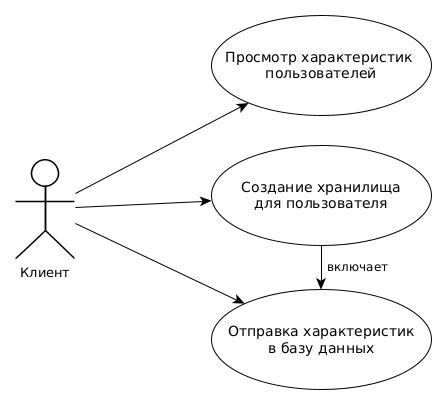
\includegraphics[scale=0.5]{img/useCase.png}
	\caption{Диаграмма вариантов использования для пользователя. }
	\label{fig:useCase}
\end{figure}

\begin{figure}[H]
	\centering
	\includegraphics[scale=0.5]{img/useCaseServer.png}
	\caption{Диаграмма вариантов использования для репозитория. }
	\label{fig:useCaseRepo}
\end{figure}

\subsection{Схема работы сервера}
На рисунке \ref{fig:serverScheme} предоставлена схема работы сервера и алгоритма обработки запросов пользователей.

\begin{figure}[hbtp]
	\centering
	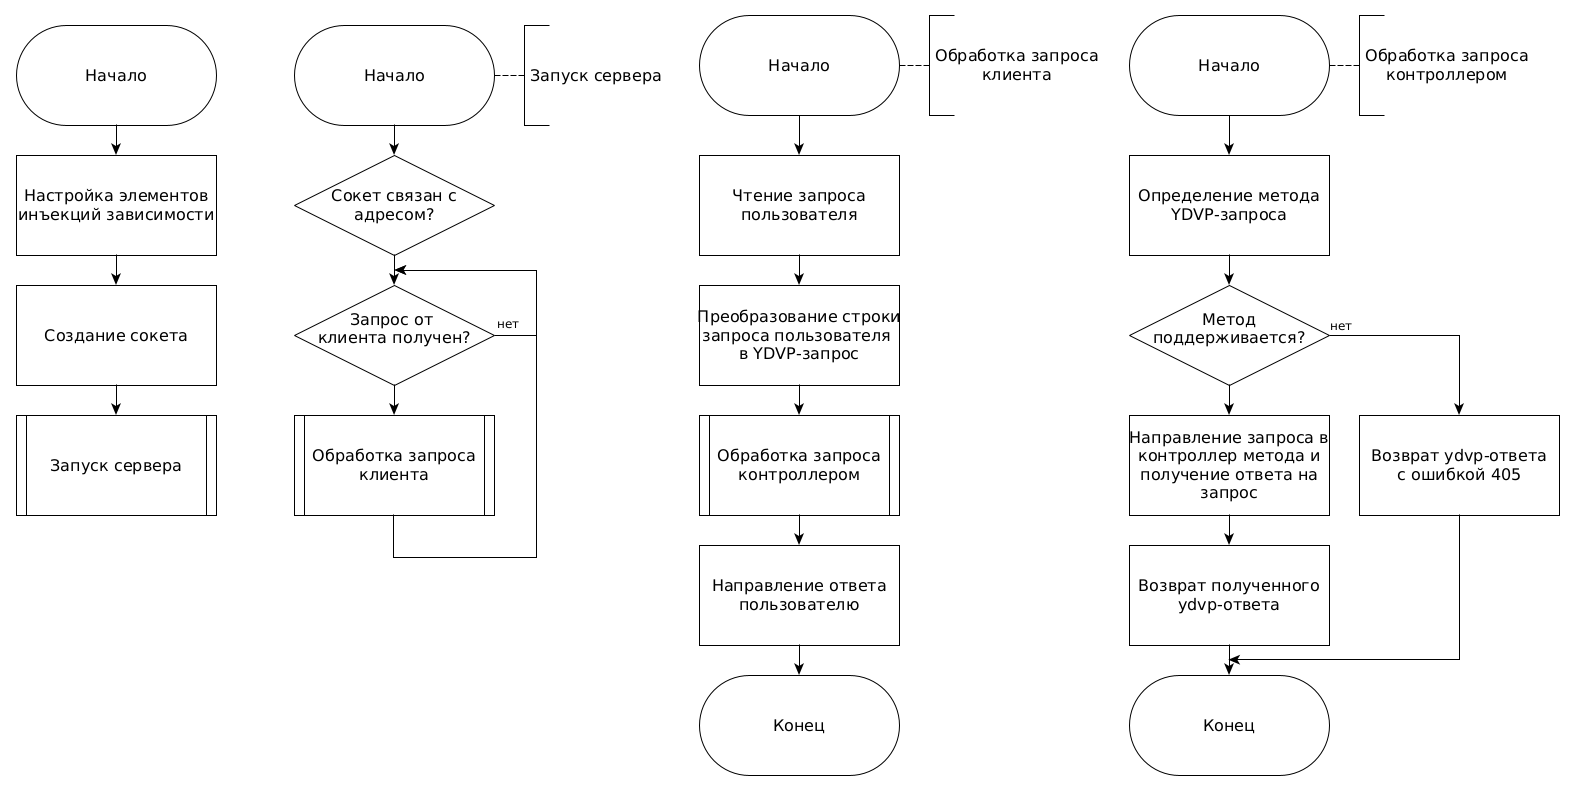
\includegraphics[width=\textwidth]{img/serverScheme.png}
	\caption{Схема работы сервера приложения. }
	\label{fig:serverScheme}
\end{figure}

\subsection{Описание YDVP-протокола}
На основе существующего стандарта HTTP в данном подразделе описывается структура реализуемого YDVP-протокола.

YDVP-запрос и YDVP-ответ включают в себя три компонента:
\begin{itemize}[leftmargin=1.6\parindent]
\item стартовую строку (определяющей тип сообщения);
\item заголовки (характеризующих тело сообщения, параметры передачи и т.д.);
\item тело (данные сообщения).
\end{itemize}

Стартовая строка запроса включает в себя:
\begin{itemize}[leftmargin=1.6\parindent]
\item метод (тип запроса);
\item путь к запрашиваемому ресурсу;
\item версию используемого протокола.
\end{itemize}

Метод указывает на основную операцию над ресурсом. При этом в качестве используемых в версии 0.1 могут быть задействованы лишь методы GET и POST, отвечающие требованиям, определенным в формализации задачи. В последующих версиях список доступных методов может быть расширен.

Стартовая строка ответа на запрос включает в себя:
\begin{itemize}[leftmargin=1.6\parindent]
\item версию используемого протокола;
\item код состояния (определяющее дальнейшее содержимое сообщения и поведение клиента);
\item пояснение к коду состояния.
\end{itemize}

Код состояния определяется по спецификации HTTP.

\subsubsection*{Вывод}
В разделе была предоставлена диаграмма вариантов использования, позволившая выделить операции, доступные клиенту и серверу. Также была предоставлена схема работы сервера, что позволило выделить основные компоненты, действующие в системе. Была описана версия 0.1 собственного протокола YDVP для взаимодействия клиента и сервера реализуемого приложения.

\pagebreak